\documentclass[11pt]{beamer}

\usetheme{metropolis}

\usepackage{graphicx}
\usepackage{physics}
\usepackage{adjustbox}
\usepackage{caption}
\usepackage{chemformula}
\usepackage{quoting}
\usepackage[style=chem-angew,backend=bibtex]{biblatex}
\bibliography{references}
%
% Choose how your presentation looks.
%
% For more themes, color themes and font themes, see:
% http://deic.uab.es/~iblanes/beamer_gallery/index_by_theme.html
%
\mode<presentation>
{
  \usetheme{default}      % or try Darmstadt, Madrid, Warsaw, ...
  \usecolortheme{default} % or try albatross, beaver, crane, ...
  \usefonttheme{default}  % or try serif, structurebold, ...
  \setbeamertemplate{navigation symbols}{}
  \setbeamertemplate{caption}[numbered]
  \setbeamerfont{footnote}{size=\tiny}
} 

\usepackage[english]{babel}
\usepackage[utf8]{inputenc}
\graphicspath{{image/}}

\AtBeginSection[]{
\begin{frame}{Outline}
  \tableofcontents[currentsection]
\end{frame}
}

\title{Chapter 2: Atoms, Ions, and the Periodic Table}
\institute{Chemistry Department, Cypress College}
\date{August 29, 2022}

\begin{document}

\begin{frame}
  \titlepage
\end{frame}

\begin{frame}{Lecture and Lab Weekly Agenda}
  \textbf{Lab Section}

  \begin{itemize}
  \item Lab lockers and safety quiz
  \item Start Exp 1 - Laboratory Techniques
  \item Using Bunsen burners
  \end{itemize}

  \textbf{Lecture Section}

  \begin{itemize}
  \item Finished Ch 1 - pg $1 - 55$
  \item Go over Ch 2 - pg $56 - 88$
  \item In-class Ch 2 worksheet
  \end{itemize}
\end{frame}

\begin{frame}{Bunsen Burner}
  \begin{columns}
    \column{0.5\textwidth}
    \centering
    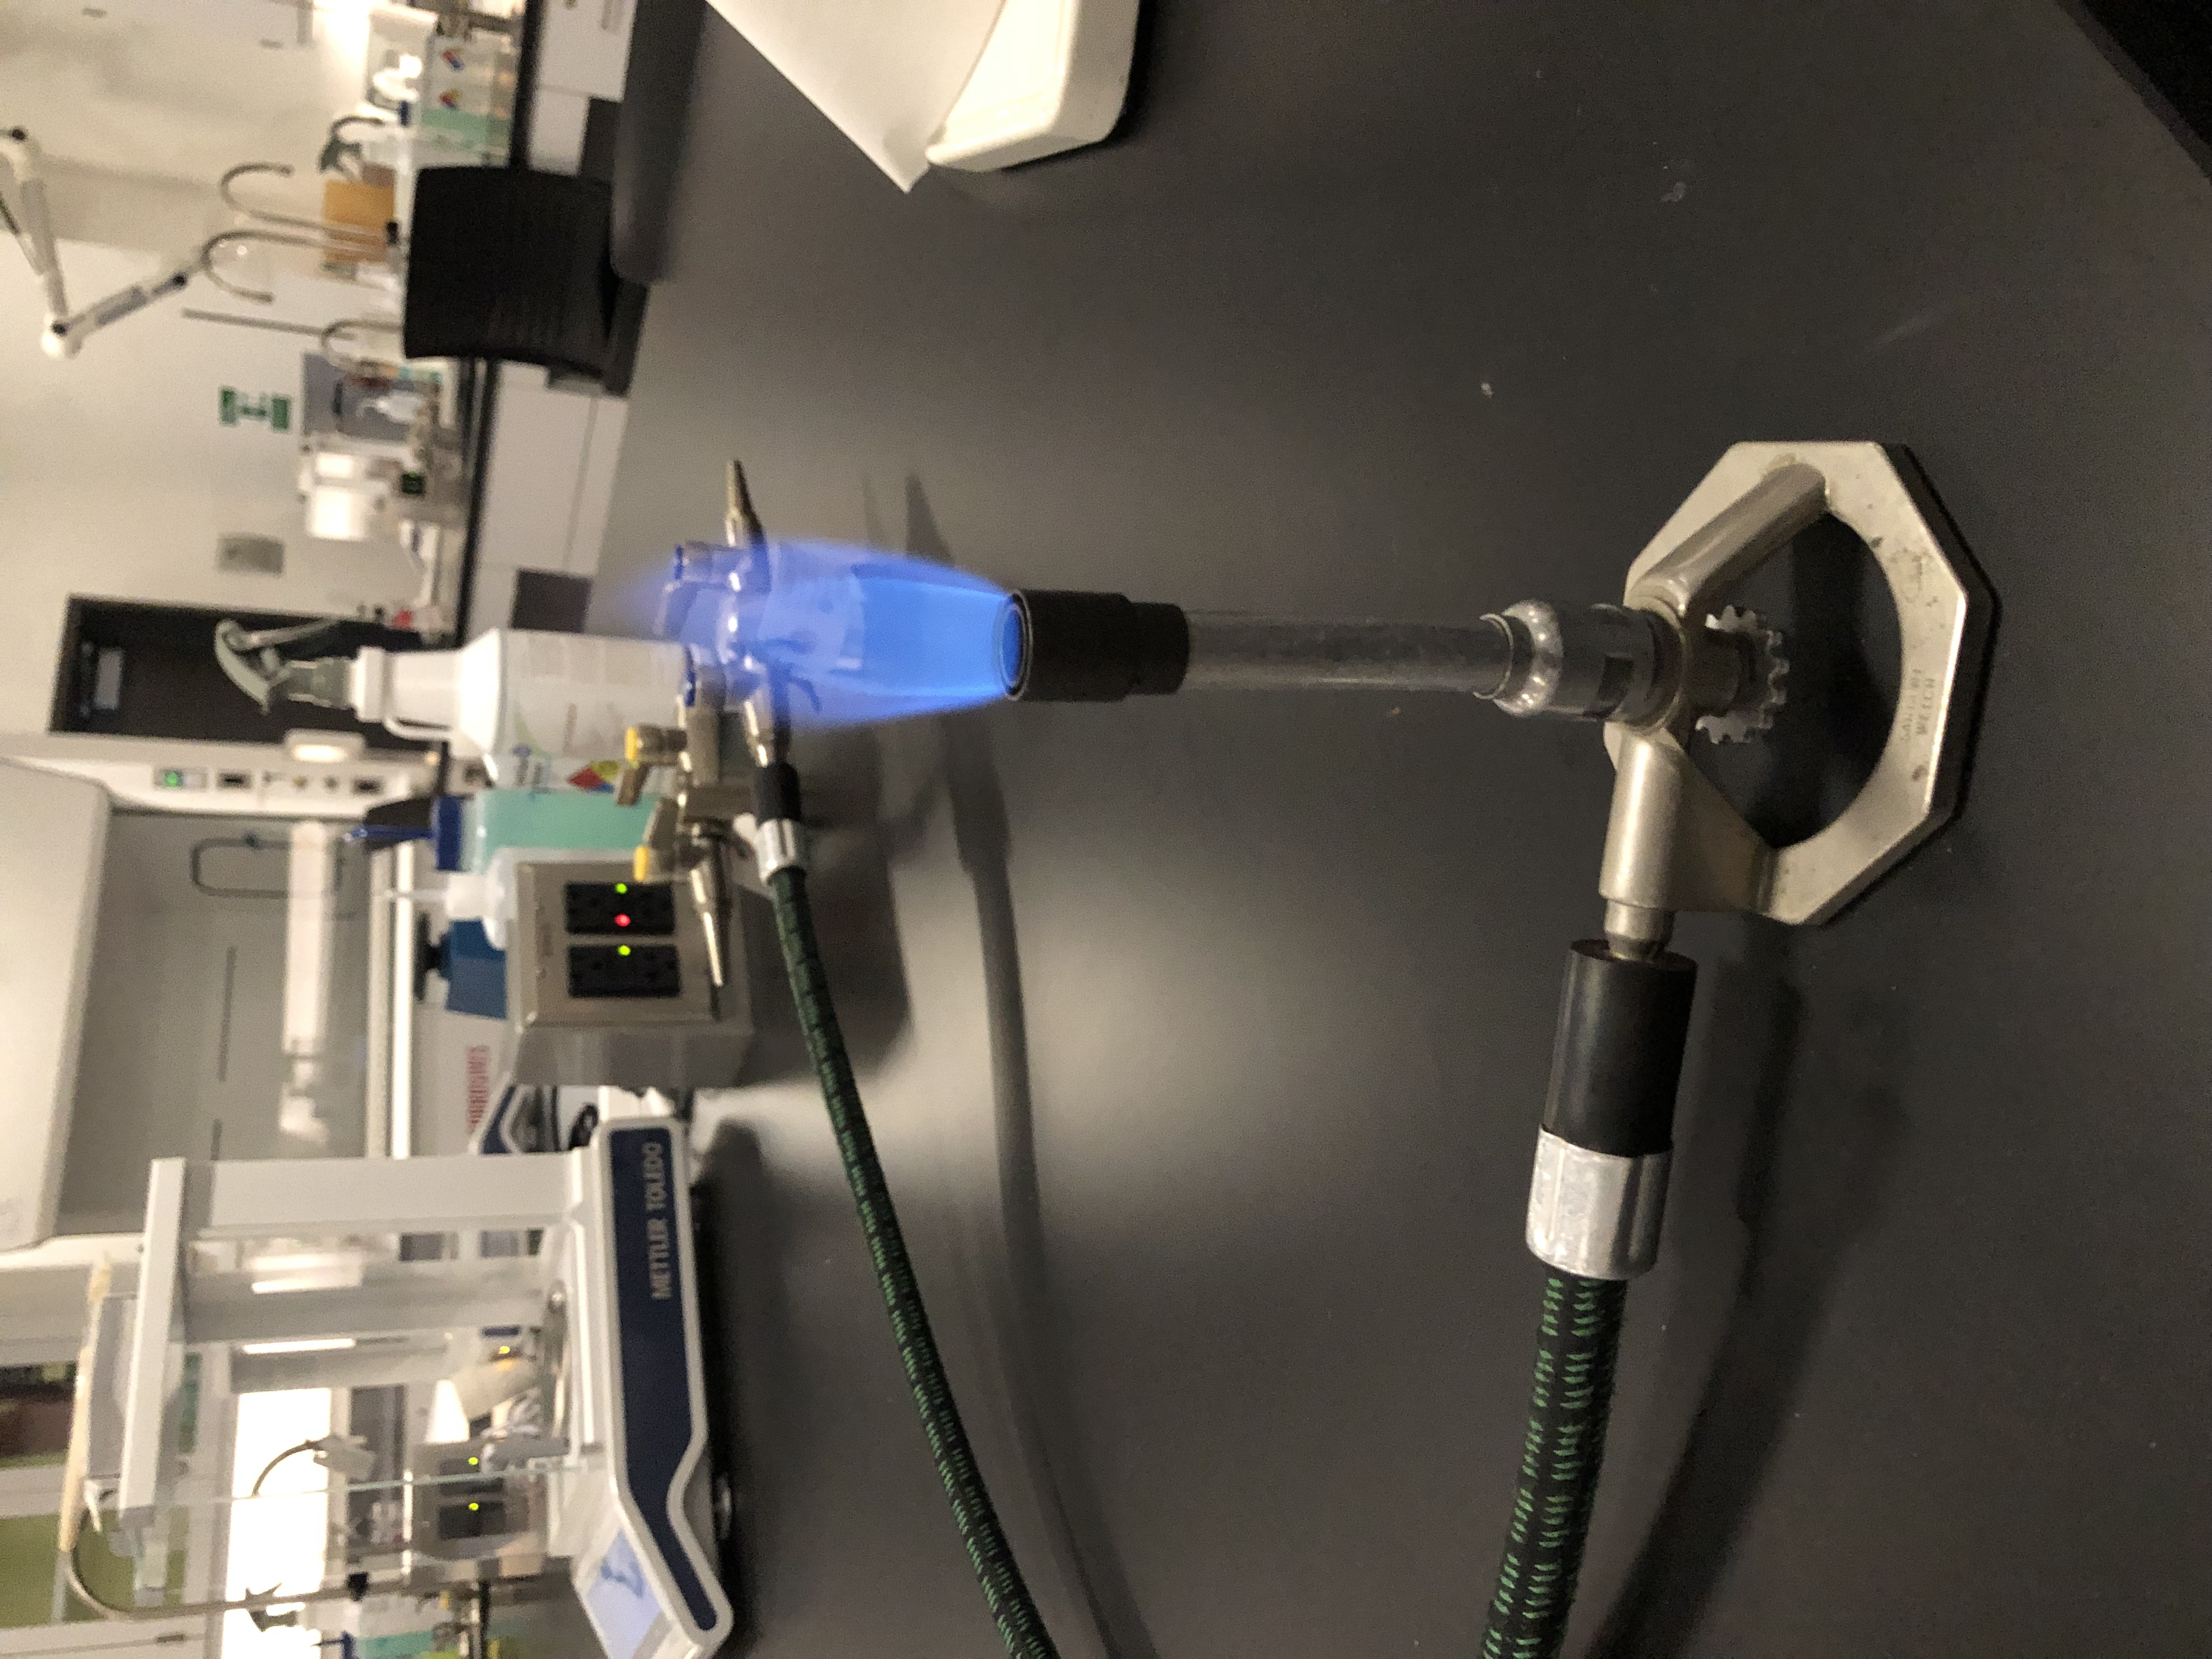
\includegraphics[angle=-90,scale=0.05]{bunsen_burn}

    \column{0.5\textwidth}
    \begin{itemize}
    \item Each student will practice lighting a
      bunsen burner under supervision
    \item Safety goggles are available (free)
    \item Review proper use of bunsen burner -
      read the lab manual
    \end{itemize}
  \end{columns}
\end{frame}

\begin{frame}{Corrections to Lecture 3}
  \begin{itemize}
  \item There is conservation of energy
  \item Amount of energy to do work is not 100$\%$
  \item Scientific notation:
    \begin{align}
      1.0\times 10^{-2}\text{g} - 1.2\times 10^{-3}\text{g}
    \end{align}
  \item Quiz - typos and mistakes on the quiz
  \end{itemize}
\end{frame}

\section{Review: Relative Atomic Mass}

\begin{frame}{Experiment: Mass Spectroscopy}
  \begin{center}
    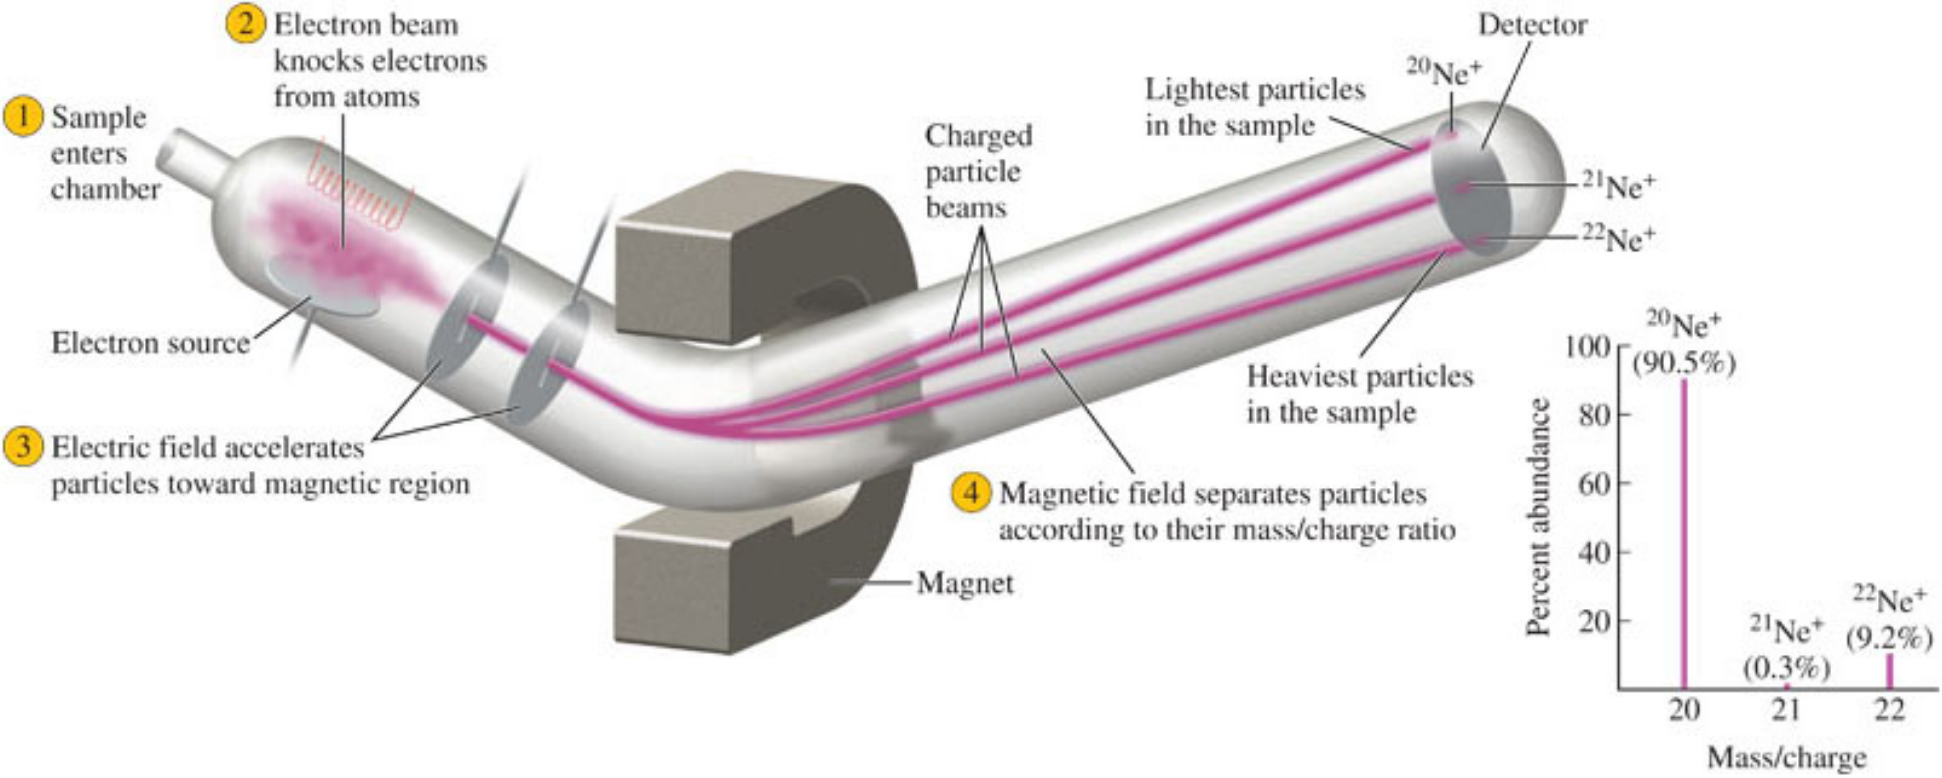
\includegraphics[width=\linewidth]{mass_spect}
  \end{center}

  \begin{itemize}
  \item Ionizes the atom and electric field accelerates atoms
  \item Time of flight - heavier atoms will travel slower
    than lighter ones
  \item Weighted average of atomic masses
  \end{itemize}  
\end{frame}

\begin{frame}{Relative Atomic Mass}
  \begin{equation}
    \text{Relative Atomic Mass} = (I_1\times A_1) + (I_2\times A_2) + \dots
  \end{equation}
  where $I$ is the mass of the isotope, and $A$ is the
  relative abundance between 0 and 1
\end{frame}

\begin{frame}{Carbon Isotopes}
  \begin{center}
    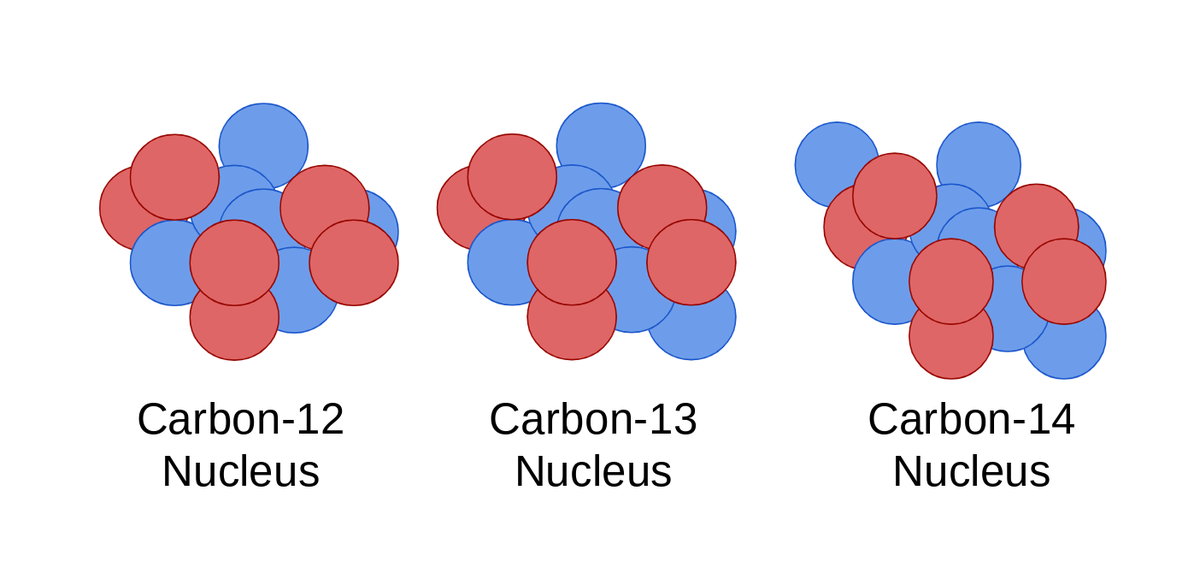
\includegraphics[scale=0.2]{carbon_isotopes}
  \end{center}
  where red is the proton and blue is the neutron
  
  \textbf{Question:} Given the carbon isotopes C-12, C-13, and C-14
  that are naturally occurring. Can you make a statement about which
  isotope is the greatest in abundance?
\end{frame}

\section{Periodic Table - Grouped Elements}

\begin{frame}{Review: Modern Period Table}
  \centering
  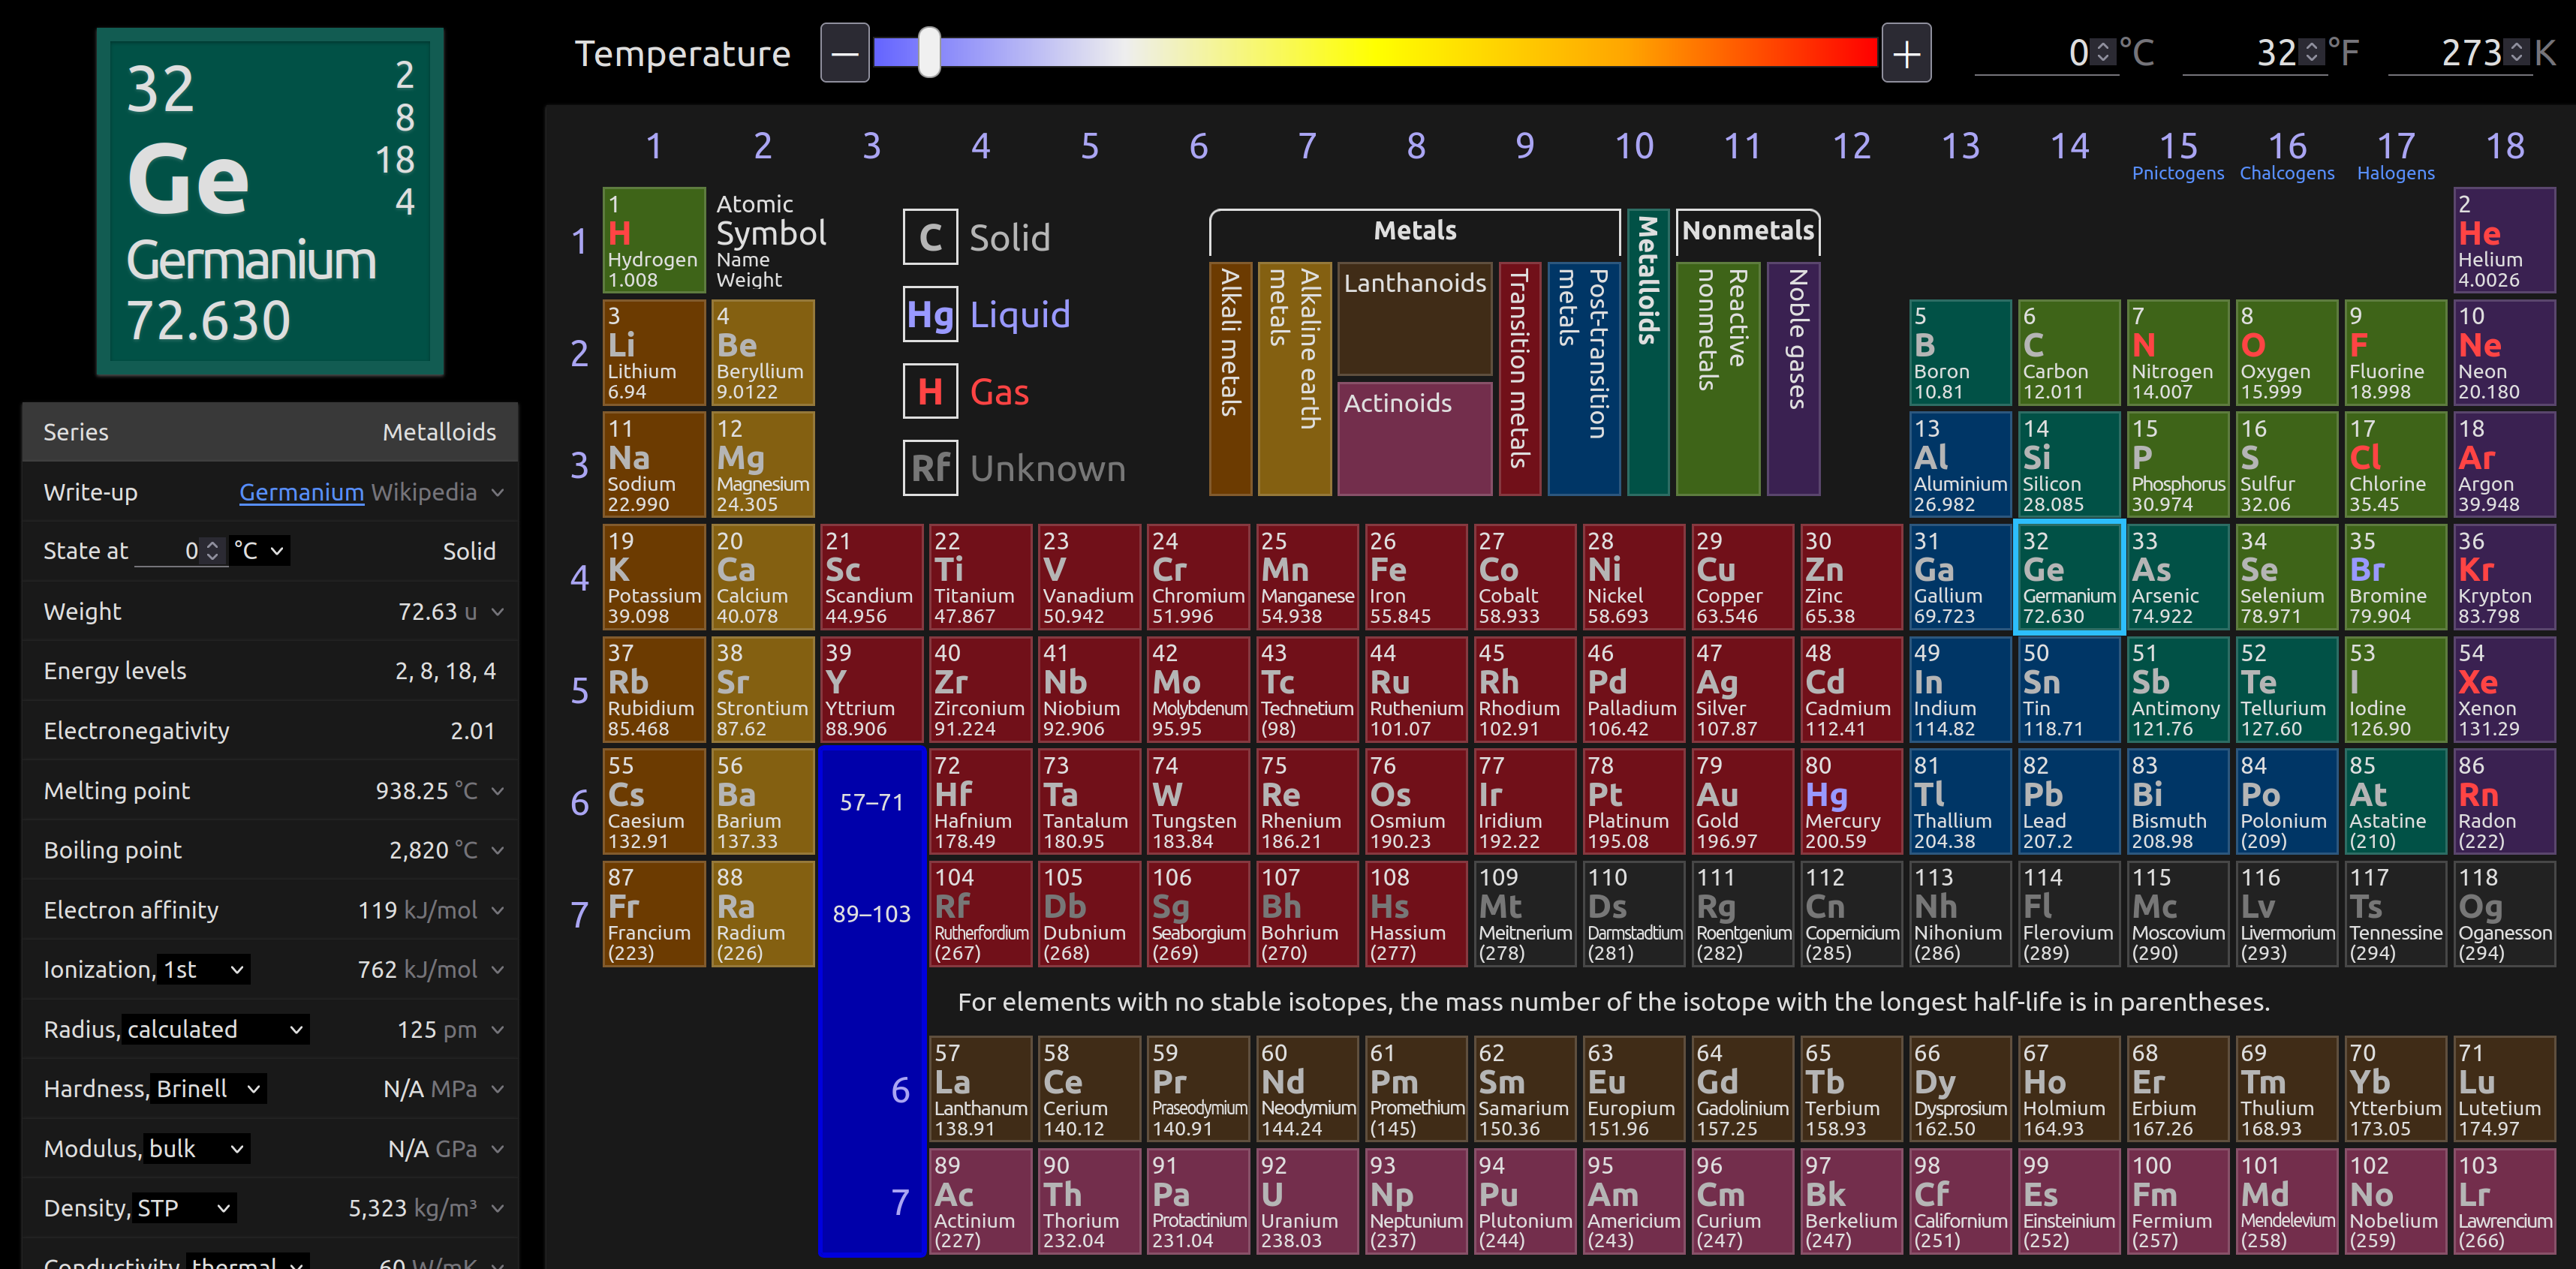
\includegraphics[width=\linewidth]{ptable}
\end{frame}

\begin{frame}{Alkali Metal}
  \begin{center}
    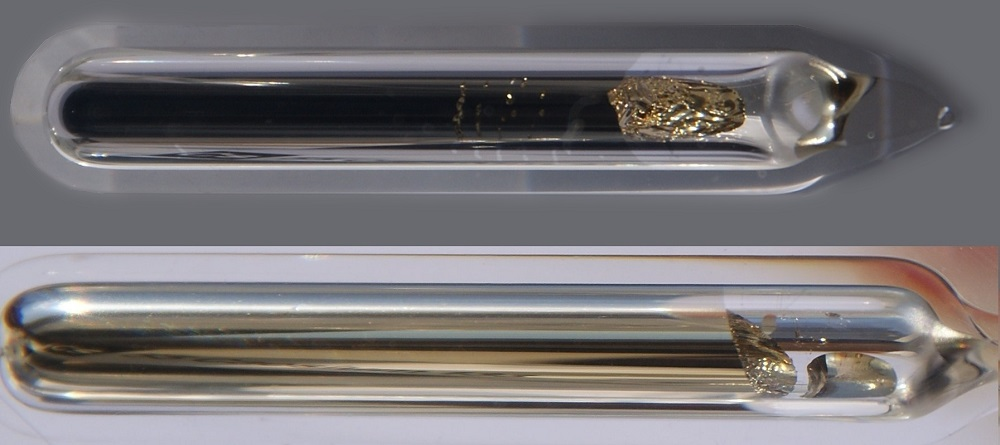
\includegraphics[scale=0.2]{alkali_metal}
  \end{center}
  
  \begin{itemize}
  \item Lower densities than other metals
  \item Extremely soft metals
  \item Highly reactive e.g. forming H$_2$ when in
    contact with water
  \item Prefer to lose an electron
  \end{itemize}
\end{frame}

\begin{frame}{Alkaline Earth Metal}
  \begin{center}
    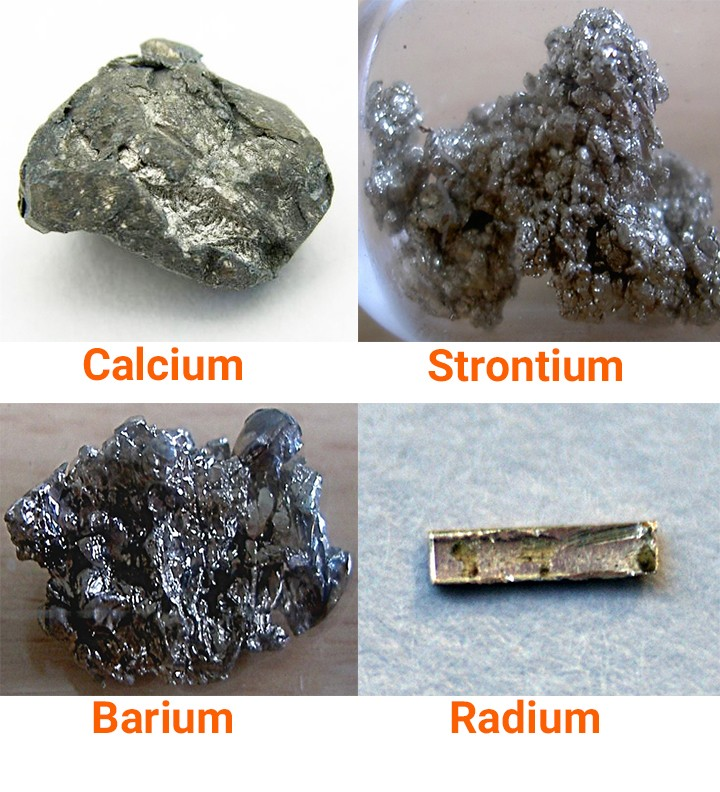
\includegraphics[width=0.4\linewidth]{alkaline_metal}
  \end{center}
  
  \begin{itemize}
  \item Fairly reactive metals
  \item Can form solutions with a pH greater than
    7 (more basic or alkaline)
  \item Calcium and magnesium important for life
  \item Prefer to lose 2 electrons
  \end{itemize}
\end{frame}

\begin{frame}{Transition Metals}
  \begin{center}
    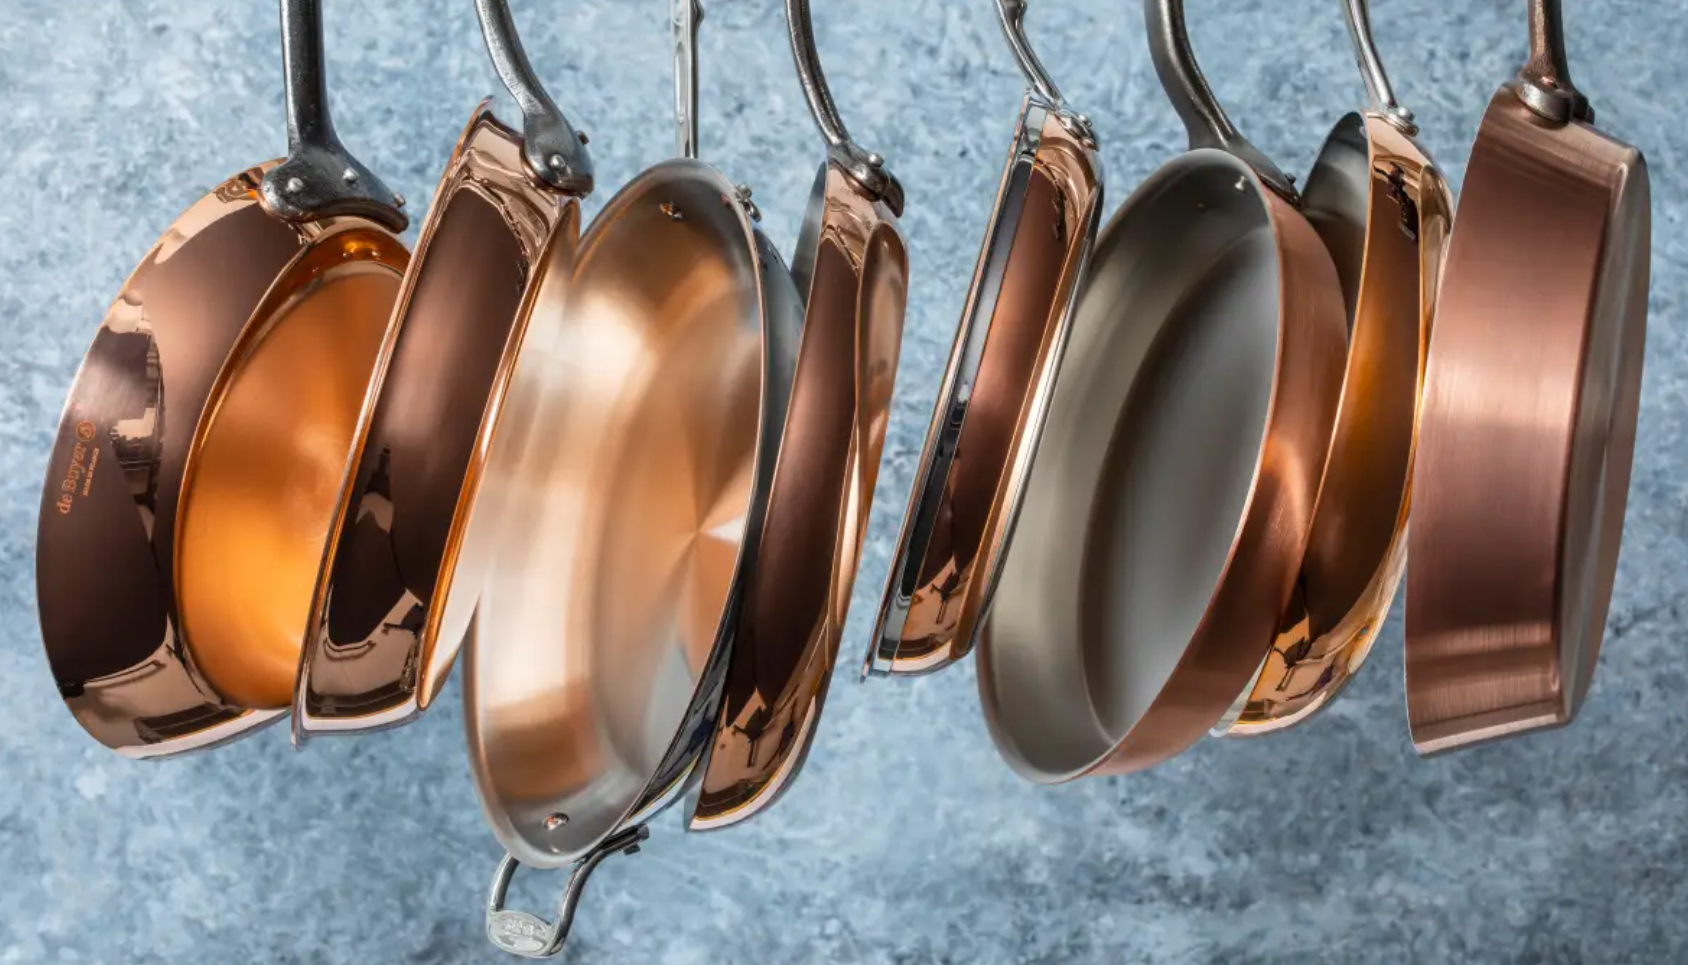
\includegraphics[scale=0.12]{copper_pan}
  \end{center}
  
  \begin{itemize}
  \item Easily malleable and great conductors of heat and
    electricity
  \item High melting points except mercury (liquid at Room
    temperature)
  \item High densities
  \item Oxidation states (ability to gain/lose electrons) can
    vary between 1+ to 6+
  \end{itemize}
\end{frame}

\begin{frame}{Actinides and Lanthanides}
  \begin{center}
    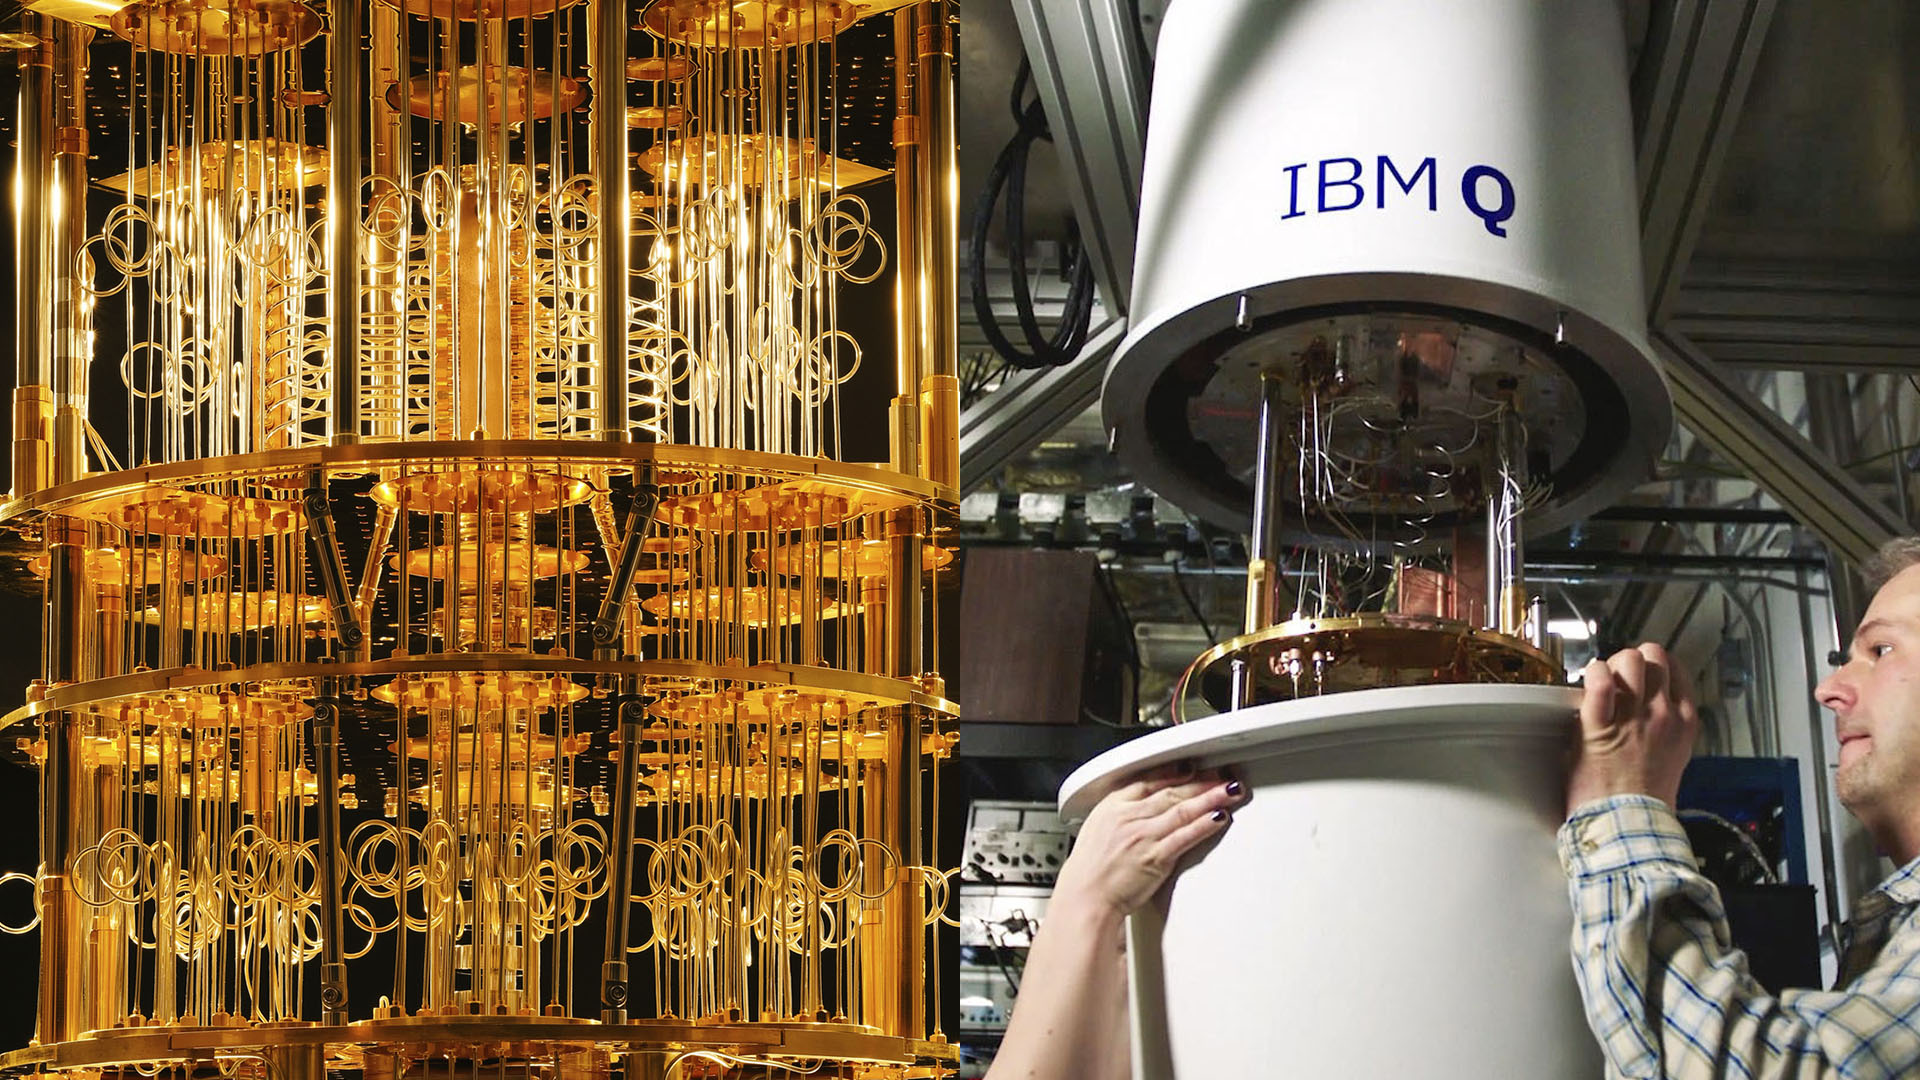
\includegraphics[scale=0.3]{quantum_comp}
  \end{center}

  \begin{itemize}
  \item Radioactive due to instability
  \item Silvery/silvery-white luster in metallic form
  \item Potential application to quantum computers and
    nuclear power
  \item Oxidation states can range from 2+ to 7+
  \end{itemize}
\end{frame}

\begin{frame}{Materials for Quantum Computing: Lanthanide Complexes}
  \begin{columns}
    \column{0.4\textwidth}
    \centering
    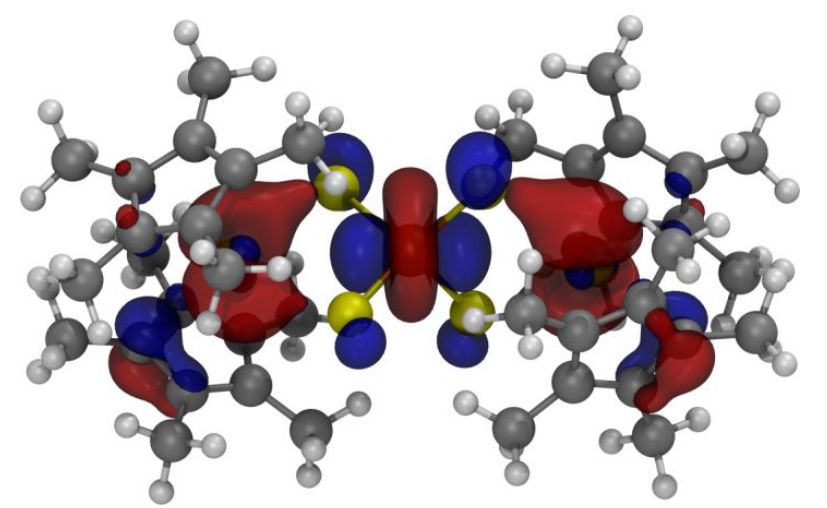
\includegraphics[scale=0.15]{gd_homo}
    \textbf{[1-Gd]$^{-1}$} HOMO
    
    \column{0.7\textwidth}
    \centering
    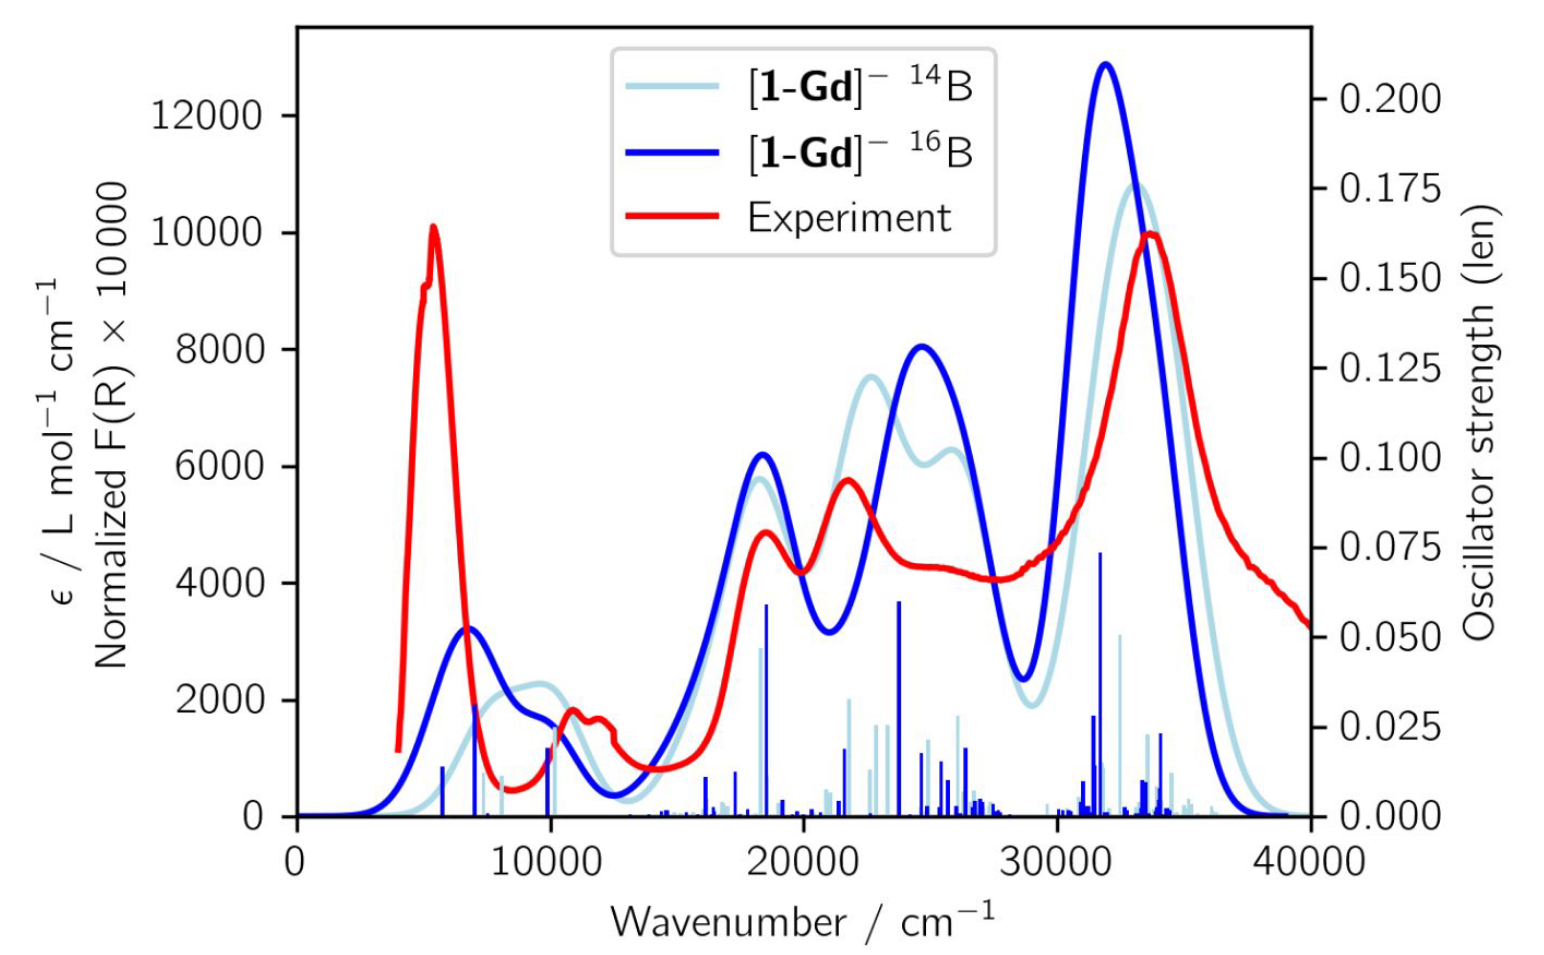
\includegraphics[scale=0.14]{gd_uv}
  \end{columns}

  \begin{itemize}
  \item Understanding the electronic structure
  \item Hysteresis - electronic spin memory
  \item \href{https://pubs.acs.org/doi/10.1021/jacs.1c03098}
    {Lanthanide MoS$_4$ research article}
  \end{itemize}
\end{frame}

\begin{frame}{Nuclear Power Plants}
  \begin{center}
    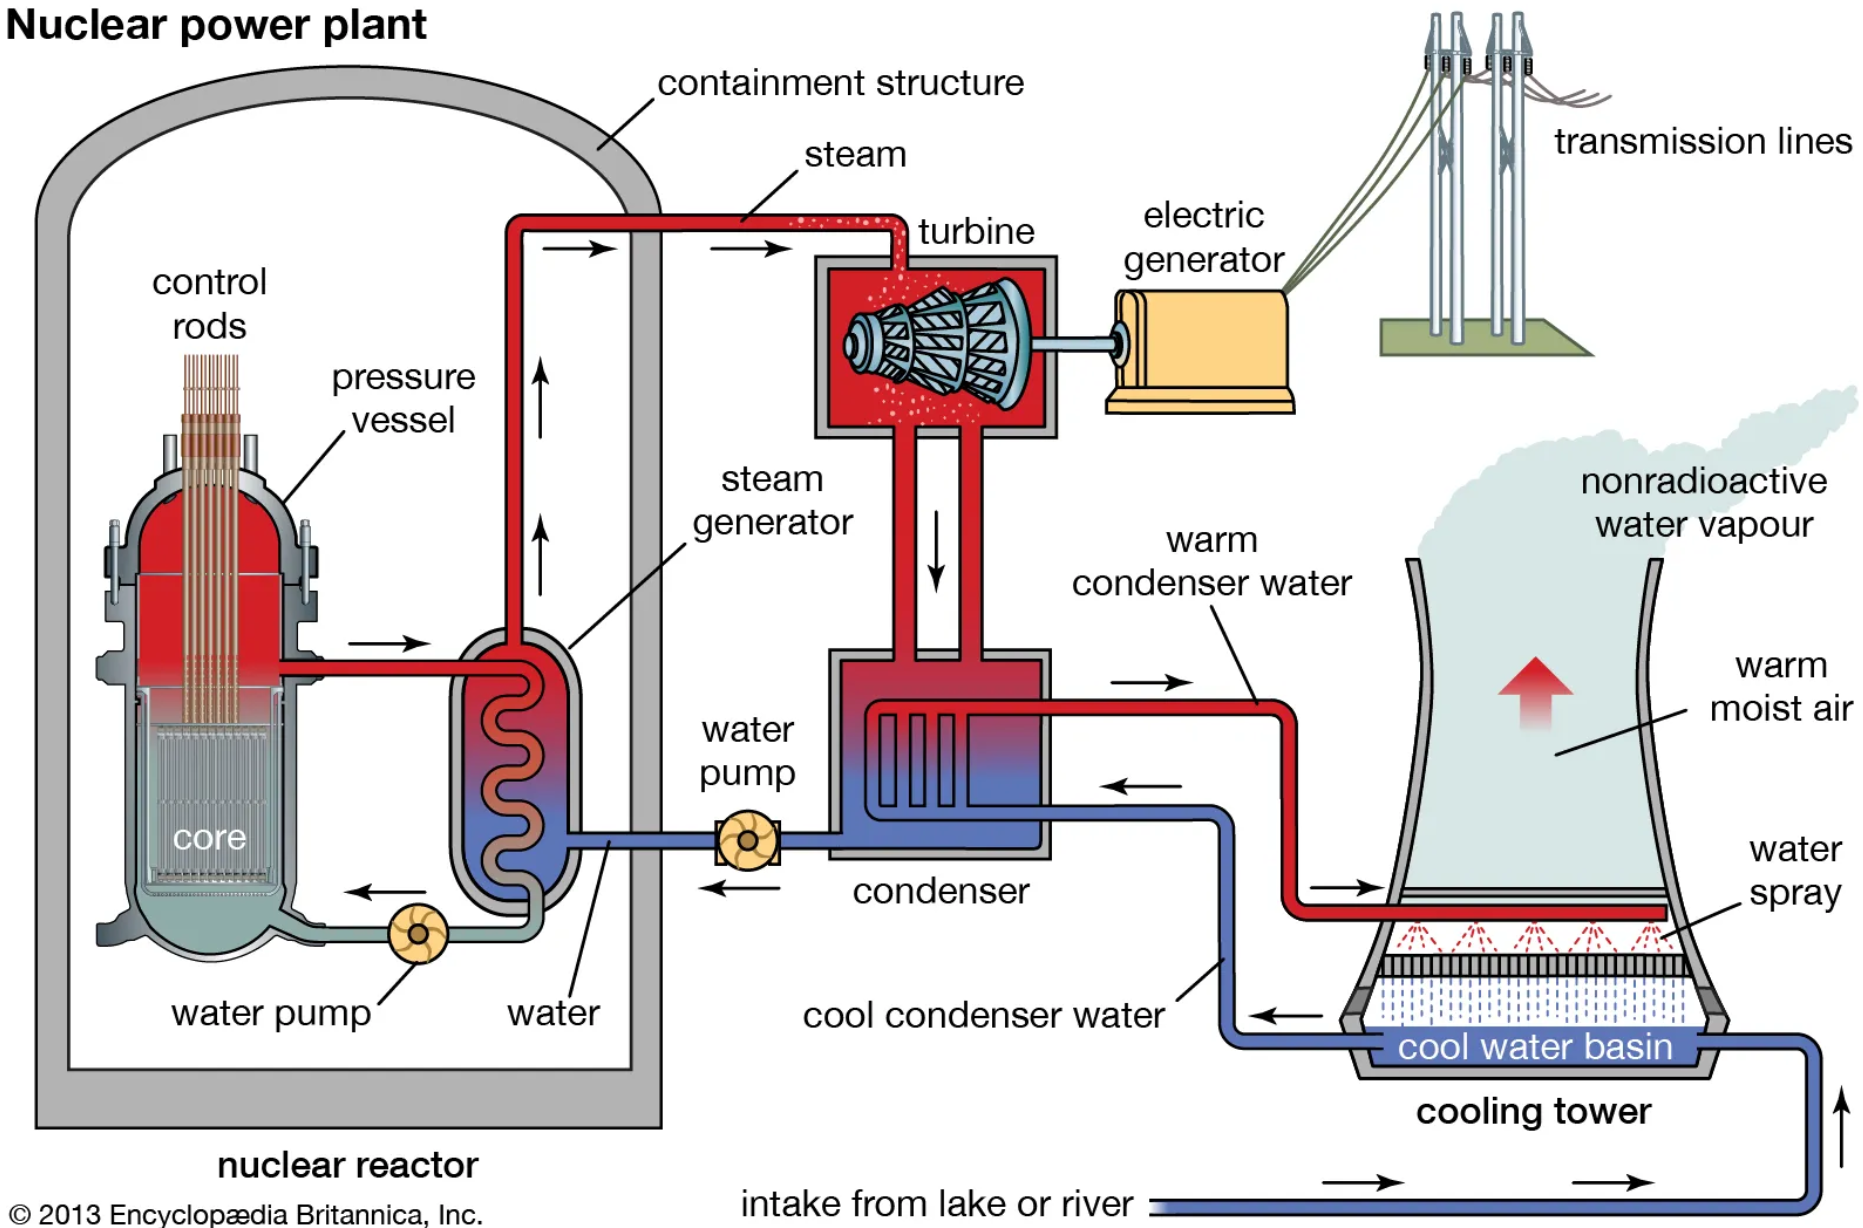
\includegraphics[width=\linewidth]{nuclear_plant}
  \end{center}
\end{frame}

\begin{frame}{Halogens}
  \begin{itemize}
  \item Fairly toxic and form acids when combined with
    hydrogen
  \item Readily react with metals to form salts e.g.
    NaCl
  \item Important for drug development due to their ``sticky''
    nature
  \item Prefers to gain an electron
  \end{itemize}
\end{frame}

\begin{frame}{Cancer Therapeutics}
  \begin{center}
    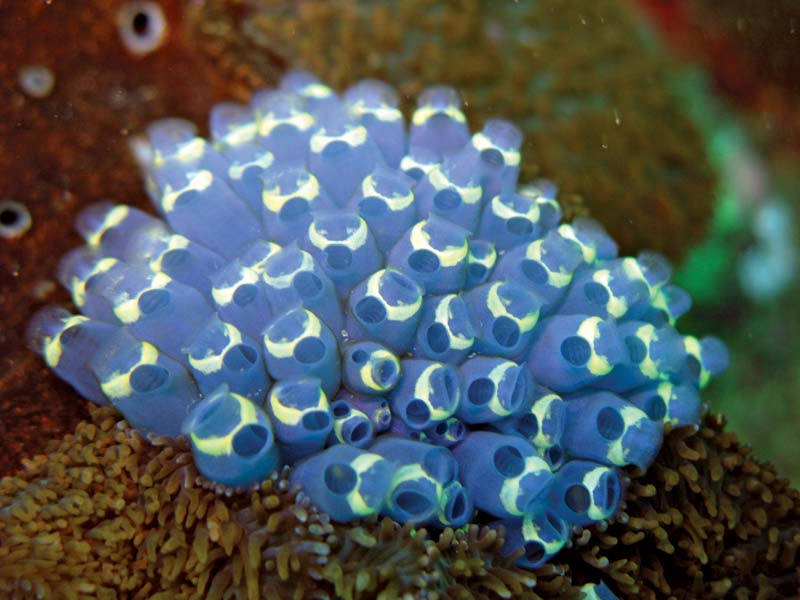
\includegraphics[scale=0.17]{sea_squirt.jpg}
  \end{center}

  \begin{itemize}
  \item Chlorolissoclimide is a potent cancer drug that
    is naturally found in sea squirts
  \item Understanding the structure--activity relationships
    e.g. interactions between drug and ribosome
  \end{itemize}
\end{frame}

\begin{frame}{My Research Project: Chlorolissoclimide}
  \begin{center}
    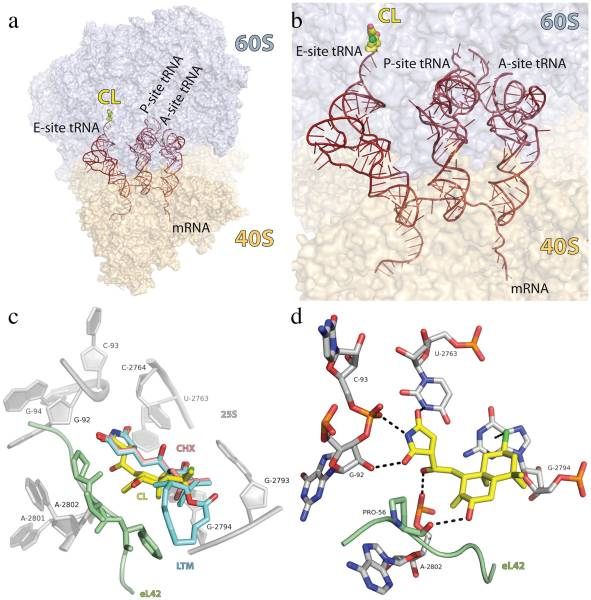
\includegraphics[trim={0 4.2in 0 0},clip,scale=0.4]{lisso_drug}
  \end{center}

  \begin{itemize}
  \item \href{https://www.nature.com/articles/nchem.2800}
    {Chlorolissoclimide research article}
  \end{itemize}
\end{frame}

\begin{frame}{Noble Gases}
  \begin{center}
    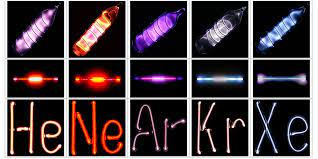
\includegraphics[scale=0.7]{neon_lights}
  \end{center}
  
  \begin{itemize}
  \item Colorless, odorless, tasteless, and non-flammable
    under standard conditions
  \item Extremely non-reactive and most stable elements
  \item Do not like to gain or lose electrons
  \end{itemize}
\end{frame}

\begin{frame}{Practice: Periodic Table}
  Group the elements into the following groups
  \begin{itemize}
  \item Br
  \item K
  \item Mg
  \item Al
  \item Mn
  \item Ar
  \item U
  \end{itemize}
\end{frame}

\begin{frame}{Practice}
  What is the charge of the ions for each of the following elements?

  \begin{itemize}
  \item Al
  \item P
  \item Br
  \item S
  \end{itemize}
\end{frame}

\end{document}
